% !TEX program = xelatex
% Disentanglement paper (paper 3).
% Build:  xelatex main && bibtex main && xelatex main && xelatex main
% Requires XeLaTeX + a Syriac-capable font (Noto Sans Syriac). If that font is
% absent, comment out the \newfontfamily\syriacfont line; the \syr macro then
% falls back to the main font (Syriac may not render; transliteration still does).

\documentclass[11pt]{article}

\usepackage[margin=1in]{geometry}
\usepackage{amsmath,amssymb}
\usepackage{booktabs}
\usepackage{array}
\usepackage{multirow}
\usepackage{graphicx}
\usepackage{microtype}
\usepackage[round]{natbib}
\usepackage[hidelinks]{hyperref}
\usepackage{xcolor}

% --- Fonts / Syriac support (XeLaTeX) ------------------------------------ %
\usepackage{fontspec}
\newfontfamily\syriacfont[Script=Syriac]{Noto Sans Syriac}
\providecommand{\syriacfont}{}
\providecommand{\RL}[1]{#1}

\newcommand{\syrscript}[1]{{\syriacfont\RL{#1}}}
\newcommand{\syr}[3]{\syrscript{#1}~(\textit{#2}, `#3')}
\newcommand{\syrt}[2]{\syrscript{#1}~(\textit{#2})}

\newcommand{\auc}{\textsc{auc}}
\newcommand{\R}{\textsc{r}}
\newcommand{\Pp}{\textsc{p}}

% The bidi package must be loaded LAST.
\usepackage{bidi}

\title{Templatic Morphology as a Disentanglement Probe:\\
Separability, a Random-Network Control, and a Causal Test of Use\\
in Frozen Encoders}

\author{Anonymous\\ \texttt{TODO: affiliation} \and Anonymous\\ \texttt{TODO: affiliation}}
\date{\today}

\begin{document}
\maketitle

\begin{abstract}
Whether a neural encoder stores distinct linguistic factors in distinct linear
subspaces---disentanglement---is hard to measure because clean, independent factor
labels are rarely available. Root-and-pattern (templatic) morphology supplies
them: every word is a product of a lexical root and a morphosyntactic pattern, and
a morphological lexicon labels both. We use this to build a balanced,
\emph{decorrelated} grid---one form per factor value per lexeme, so lexical
identity is statistically independent of the factor---and measure a $2\times2$
cross-erasure selectivity matrix: can a linear projection erase one factor while
the other survives, in both directions? On Classical Syriac (from the SEDRA
lexicon) the matrix is clean across three morphosyntactic factors (number, gender,
state) and three frozen encoders, including a byte model never trained on Syriac:
erasing the factor sends its probe to chance while lexeme retrieval is untouched,
and erasing lexical identity leaves the factor decodable. INLP and the closed-form
LEACE agree. Crucially, a \textbf{random-initialised} encoder of the same
architecture reproduces both the decodability and the clean off-diagonal (number
$0.78$ vs.\ $0.83$ pretrained), so this separability is substantially a property of
the surface form and the byte architecture rather than something pretraining
discovers---a control-task caution that the instrument makes quantifiable. What
pretraining and in-language adaptation \emph{do} add is measurable but modest:
higher absolute decodability and a sharper relocation of number into the vocalic
channel (a consonantal control localises each factor to where the script writes
it). The geometry, however, is not the whole story: a causal intervention on
Hebrew agreement---erasing a feature's subspace and reading the effect off the
model's own masked-LM head---shows a clean double dissociation in the pretrained
model (erasing number collapses number agreement to chance while sparing gender,
and vice versa) that is \emph{absent} from the random network, which has no
agreement to break. The separability is surface-carried, but the \emph{use} of it
is learned. The design replicates on Hebrew and Arabic via UniMorph. We argue that
templatic morphology is a reusable instrument for representation-geometry
questions, that its random-network baseline is as much of the result as the effect,
and that a behavioural intervention is what separates shape from use.
\end{abstract}

% ===================================================================== %
\section{Introduction}
\label{sec:intro}

A recurring question in interpretability is whether a representation is
\emph{disentangled}: are separate factors of variation stored along separate,
independently manipulable directions? The question is notoriously hard to answer,
and a central reason is measurement. To test whether factor $A$ is encoded
separately from factor $B$, one needs many examples in which $A$ and $B$ vary
independently and both are labelled; otherwise a probe for $A$ may be reading $B$,
or a shared confound such as lexical frequency. Clean, independent factor labels at
scale are exactly what most natural data lacks, and unsupervised disentanglement
without them is provably under-determined \citep{locatello2019challenging}.

Root-and-pattern morphology offers an unusual escape. In a templatic Semitic
language a word is, almost literally, a product of two factors: a consonantal
\emph{root} that carries lexical identity and a vocalic/affixal \emph{pattern} that
carries morphosyntax. A morphological lexicon labels both factors for every form.
This lets us construct a \emph{balanced, decorrelated} probe set: take every lexeme
attested with both values of a binary factor (e.g.\ singular and plural) and keep
exactly one form per value, so that across the set the factor is statistically
independent of lexical identity by construction. On such a set we can ask the
disentanglement question directly and symmetrically.

Our instrument is a $2\times2$ \emph{cross-erasure selectivity matrix}. We probe a
frozen encoder for the factor and, separately, retrieve lexical identity by nearest
neighbour. We then linearly erase each in turn---erase the factor and re-measure
both; erase identity and re-measure both. A clean off-diagonal (erasing the factor
leaves identity, erasing identity leaves the factor) is the signature of two
separable linear subspaces.

Applied to Classical Syriac the matrix is clean, and it stays clean across three
factors, three encoders, and---via UniMorph---Arabic and Hebrew. But the
contribution we want to stress is what a control reveals. A \textbf{random-init}
encoder of the same architecture, with no training at all, reproduces the clean
matrix almost entirely. The separability is therefore substantially a property of
the \emph{surface form}---a random byte network is a random feature map over
character $n$-grams, and templatic morphology marks the factor in consistent
affixal/vocalic positions that such a map preserves---rather than something
pretraining had to learn. This is a control-task lesson \citep{hewitt2019control} that
the instrument turns into a number. What pretraining and in-language adaptation add
is real but modest, and the same instrument measures it: higher absolute
decodability, and a sharper relocation of the number signal into the vowels, which
a consonantal control isolates.

\paragraph{Contributions.}
\begin{enumerate}
  \item \textbf{Templatic morphology as a disentanglement instrument.} We turn the
  root/pattern factorisation of a Semitic lexicon into a balanced, decorrelated
  probe set and a symmetric cross-erasure selectivity matrix
  (\S\ref{sec:instrument},~\S\ref{sec:method}). It needs no model training and no
  synthetic data.
  \item \textbf{Frozen encoders linearly separate pattern from identity}, cleanly,
  across three morphosyntactic factors and three encoders---including one never
  trained on the language---confirmed by both INLP and closed-form LEACE and stable
  across seeds (\S\ref{sec:syriac}).
  \item \textbf{A random-network control that reframes the effect.} The same matrix
  is reproduced by a random-init encoder, so the separability is largely
  surface-carried; we quantify what pretraining and Syriac adaptation add on top---a
  modest sharpening and a relocation of number into the vocalic channel, the latter
  isolated by a consonantal control (\S\ref{sec:controls}).
  \item \textbf{A causal dissociation that separates shape from use.} On Hebrew
  agreement, read from the model's own masked-LM head, erasing a feature's subspace
  collapses \emph{only} that feature's agreement to chance in the pretrained model
  (a double dissociation), while a rank-matched random direction spares both and the
  random-init network has no agreement to break (\S\ref{sec:causal}). The geometry is
  surface-carried; the function is learned.
  \item \textbf{Cross-lingual replication.} The design transfers unchanged to
  Hebrew (with a native encoder, on UniMorph labels) and extends to Arabic by the
  same minimal-pair construction, supporting the claim that this is a reusable
  instrument rather than a Syriac-specific curiosity (\S\ref{sec:crosslang}).
\end{enumerate}

% ===================================================================== %
\section{Related Work}
\label{sec:related}

\paragraph{Probing.}
Diagnostic classifiers probe a frozen representation for a property
\citep{conneau2018probing,belinkov2017morphology}, and structural probes recover
syntax \citep{hewitt2019structural}. The methodology's central hazard is that a
probe may succeed by exploiting the representation's general capacity rather than a
targeted property; \citet{hewitt2019control} introduce \emph{control tasks} (here, a
random-control representation) to calibrate this, and \citet{belinkov2022probing}
surveys the resulting cautions. Our random-init encoder is exactly such a control,
and it is the reason we frame the surface baseline as part of the result.

\paragraph{Concept erasure.}
Beyond reading a factor, one can try to remove it. Iterative nullspace projection
(INLP) repeatedly fits and projects out a linear classifier
\citep{ravfogel2020null}; amnesic probing then measures the effect of removal
\citep{elazar2021amnesic}; LEACE gives the closed-form, minimally-damaging linear
eraser \citep{belrose2023leace}. We use INLP and LEACE as the two directions of our
matrix and check that they agree.

\paragraph{Disentanglement and concept directions.}
Unsupervised disentanglement is under-determined without inductive bias or
supervision \citep{locatello2019challenging,higgins2018definition}; we sidestep the
impossibility by letting the language supply labelled, independent factors. That
morphosyntactic features occupy consistent linear directions echoes the analogy
geometry of word vectors \citep{mikolov2013linguistic} and lexical-semantic probing
of contextual encoders \citep{vulic2020probing}; morphological content in such
encoders has been studied directly \citep{edmiston2020systematic}.

\paragraph{Morphology, resources, and Semitic NLP.}
Our factor labels come from the SEDRA Syriac lexicon \citep{kiraz1994sedra} and from
UniMorph \citep{mccarthy2020unimorph} for Arabic and Hebrew; the Arabic encoder is
CAMeLBERT \citep{inoue2021camelbert} and the Hebrew encoder AlephBERT
\citep{seker2022alephbert}, with a tokenizer-free byte encoder, CANINE
\citep{clark2022canine}, for Syriac. For the language see
\citet{brock2006introduction,butts2019syriac}; a neural Syriac morphological parser
is \citet{naaijer2023transformer}. Tooling is \textsc{Transformers}
\citep{wolf2020transformers} and \textsc{NumPy} \citep{harris2020numpy}.

% ===================================================================== %
\section{The Instrument: Root \texorpdfstring{$\times$}{x} Pattern as Ground Truth}
\label{sec:instrument}

\paragraph{Factorisation.}
In a root-and-pattern language a surface form realises a lexical root through a
morphosyntactic pattern. We treat the pair (lexical identity \R, a binary
morphosyntactic factor \Pp) as two ground-truth factors of variation. For Syriac we
we take \R\ to be the SEDRA lexeme \citep{kiraz1994sedra,sedraproject} and \Pp\ one of: \emph{number} (singular vs
plural), \emph{gender} (masculine vs feminine), or \emph{state} (emphatic vs
absolute)---the three features that vary \emph{within} a lexeme and so admit a
within-lexeme contrast. Part of speech, which does not vary within a lexeme, cannot
serve.

\paragraph{A balanced, decorrelated grid.}
For a factor \Pp\ we keep every lexeme attested with both values and sample exactly
one form per value. The resulting grid has each lexeme appearing once per factor
value, so \Pp\ is balanced $50/50$ and, across lexemes, independent of \R: a probe
for \Pp\ cannot succeed by memorising lexical identity, and identity retrieval
cannot succeed by reading \Pp. For Arabic and Hebrew we build the same grid from
UniMorph by taking \emph{minimal pairs}---two forms of a lemma whose feature bundles
differ only in \Pp---which holds every other morphosyntactic dimension fixed.

\paragraph{Surface and a consonantal control.}
Each Syriac form is available vocalised (\syrt{ܡܠܟܐ}{malk\=a}, with pointing) and as a
bare consonantal skeleton. We run the whole pipeline on both. Because Syriac writes
number partly in the vowels and gender/state mainly in the consonants, comparing
vocalised against consonantal localises \emph{where} each factor is marked, and
guards against the matrix being a trivial artefact of a single salient character.
Arabic UniMorph forms carry full diacritics, giving the same control; Hebrew
UniMorph forms are unvocalised, so there the control is vacuous and noted as such.

% ===================================================================== %
\section{Method}
\label{sec:method}

\paragraph{Encoding.}
Every form is encoded by a \emph{frozen} model as a single mean-pooled vector. For
Syriac we use off-the-shelf CANINE (a codepoint byte encoder never trained on
Syriac), the same model after light Syriac LoRA adaptation, and a Hebrew model fed
Syriac transliterated into Hebrew script. No encoder is fine-tuned for our task;
the probes and erasers are linear and operate on the frozen vectors.

\paragraph{Probes.}
We split the grid \emph{by lexeme} into train and test, so the factor probe must
generalise across lexemes rather than memorise forms. The factor probe \Pp\ is a
logistic regression; chance is $0.5$. Lexical identity \R\ is measured by
self-excluded nearest-neighbour retrieval (does a form's nearest neighbour share its
lexeme?); chance is $1/{\,}|\text{test lexemes}|$, typically $<0.01$.

\paragraph{Erasure.}
To erase the factor we use iterative nullspace projection (INLP)
\citep{ravfogel2020null} and, as a closed-form check, LEACE
\citep{belrose2023leace}, both fit on train and applied to test. To erase lexical
identity we project out the top principal directions of the lexeme-mean subspace.
Erasers are linear maps $P$ applied as $X\!\to\!XP$, so the same probe reads the
erased space. We report the $2\times2$ matrix: original, post-factor-erasure, and
post-identity-erasure, for both \Pp\ and \R. Everything is computed over five
train/test seeds and reported as mean${}\pm{}$standard deviation. Probes and erasers
are plain \textsc{NumPy}; no concept-erasure library is required.

% ===================================================================== %
\section{Frozen Encoders Separate Pattern from Identity}
\label{sec:syriac}

Table~\ref{tab:matrix} reports the selectivity matrix on vocalised Syriac. The
off-diagonal is clean in every cell. Reading the number row for off-the-shelf
CANINE: the factor is decodable at $0.83$ and collapses to chance ($0.51$) when
erased, while lexeme retrieval is untouched ($0.33\!\to\!0.36$); conversely, erasing
lexical identity drives retrieval to $0.00$ while number stays decodable at $0.77$.
The same pattern holds for gender and state and for all three encoders, including
the Hebrew-transfer model that never saw Syriac. Multi-seed standard deviations are
small ($\le 0.05$), so the structure is stable, not a single-split accident.

\begin{table}[t]
  \centering
  \small
  % Generated by disentangle/results.py -- do not edit by hand.
\begin{tabular}{llcccccc}
\toprule
& & \multicolumn{3}{c}{Factor acc.\ (chance .5)} & \multicolumn{3}{c}{Lexeme \textsc{nn}} \\
\cmidrule(lr){3-5}\cmidrule(lr){6-8}
Encoder & Factor & orig.\ & $-$factor & $-$lexeme & orig.\ & $-$factor & $-$lexeme \\
\midrule
CANINE (frozen) & number & $0.828\pm0.011$ & $0.511\pm0.015$ & $0.770\pm0.039$ & $0.333\pm0.021$ & $0.357\pm0.022$ & $0.000\pm0.001$ \\
CANINE (frozen) & gender & $0.721\pm0.032$ & $0.526\pm0.023$ & $0.650\pm0.015$ & $0.284\pm0.037$ & $0.312\pm0.039$ & $0.009\pm0.005$ \\
CANINE (frozen) & state & $0.846\pm0.031$ & $0.506\pm0.019$ & $0.799\pm0.024$ & $0.441\pm0.046$ & $0.517\pm0.031$ & $0.004\pm0.005$ \\
CANINE (Syriac LoRA) & number & $0.870\pm0.038$ & $0.502\pm0.020$ & $0.781\pm0.020$ & $0.292\pm0.021$ & $0.323\pm0.021$ & $0.000\pm0.001$ \\
CANINE (Syriac LoRA) & gender & $0.722\pm0.012$ & $0.516\pm0.043$ & $0.657\pm0.033$ & $0.207\pm0.035$ & $0.249\pm0.041$ & $0.009\pm0.005$ \\
CANINE (Syriac LoRA) & state & $0.867\pm0.022$ & $0.503\pm0.027$ & $0.759\pm0.026$ & $0.265\pm0.038$ & $0.537\pm0.047$ & $0.011\pm0.006$ \\
Hebrew transfer & number & $0.622\pm0.005$ & $0.500\pm0.025$ & $0.561\pm0.011$ & $0.352\pm0.026$ & $0.367\pm0.027$ & $0.001\pm0.003$ \\
Hebrew transfer & gender & $0.628\pm0.024$ & $0.467\pm0.041$ & $0.548\pm0.043$ & $0.253\pm0.022$ & $0.286\pm0.021$ & $0.007\pm0.004$ \\
Hebrew transfer & state & $0.821\pm0.016$ & $0.469\pm0.018$ & $0.750\pm0.070$ & $0.322\pm0.041$ & $0.397\pm0.039$ & $0.008\pm0.007$ \\
\bottomrule
\end{tabular}

  \caption{Cross-erasure selectivity matrix on vocalised Syriac (frozen encoders;
  mean${}\pm{}$SD over five seeds). Factor accuracy has chance $0.5$. A clean
  off-diagonal---erasing the factor leaves lexeme \textsc{nn} while sending factor
  accuracy to chance, and erasing the lexeme leaves factor accuracy while sending
  lexeme \textsc{nn} to zero---indicates separable linear subspaces.}
  \label{tab:matrix}
\end{table}

Figure~\ref{fig:arrow} visualises the geometry for number: projecting onto the
factor axis (the train mean difference) and an orthogonal identity axis, each
lexeme's singular and plural forms are displaced in a common direction.
Figure~\ref{fig:erase} shows the same scatter before and after erasing the factor:
the value-$0$/value-$1$ classes separate originally and intermix after erasure,
while lexical structure is preserved.

\begin{figure}[t]
  \centering
  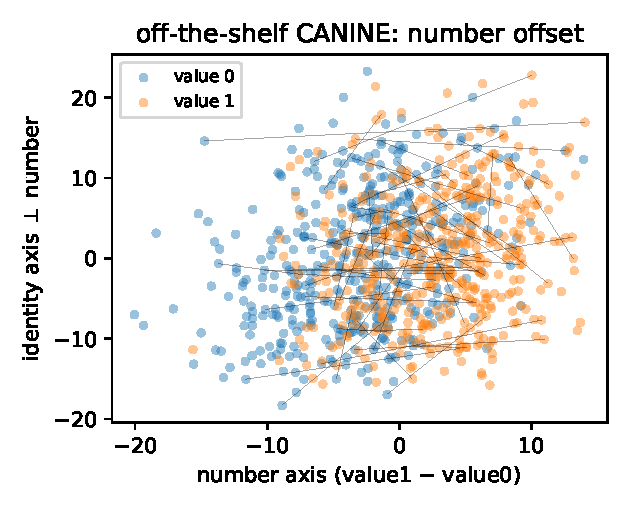
\includegraphics[width=0.62\linewidth]{figures/FD1_arrow_canine_number.pdf}
  \caption{Number offset for off-the-shelf CANINE: held-out forms on the factor
  axis (plural $-$ singular) vs.\ an orthogonal identity axis, with each lexeme's
  two forms joined. The factor is a consistent displacement.}
  \label{fig:arrow}
\end{figure}

% ===================================================================== %
\section{What the Effect Is, and What It Is Not}
\label{sec:controls}

\paragraph{A random network reproduces the matrix.}
Table~\ref{tab:floorleace} (top) runs the identical pipeline on a
\emph{random-initialised} CANINE---same architecture, same byte inputs, no
training. It does not collapse: number is decodable at $0.78$ (vs.\ $0.83$
pretrained), gender at $0.72$, state at $0.82$, and the off-diagonal stays clean
(erasing the factor still reaches chance; erasing identity still sends retrieval to
zero). The separability is therefore substantially a property of the \emph{surface
form} and the byte architecture: a random network is a random feature map over
character $n$-grams, and a templatic factor marked in consistent affixal or vocalic
positions survives such a map and stays linearly separable from identity. Read as a
control task \citep{hewitt2019control}, this is a caution---high probe accuracy and
clean erasure do not by themselves implicate the \emph{learned} representation---and
the instrument makes the caution quantitative.

\paragraph{INLP and LEACE agree.}
Table~\ref{tab:floorleace} (bottom) confirms the erasure is not an artefact of the
iterative method: the closed-form LEACE drives post-erasure factor accuracy to the
same chance level as INLP for all three factors.

\begin{table}[t]
  \centering
  \small
  % Generated by disentangle/results.py -- do not edit by hand.
\begin{tabular}{llccc}
\toprule
Setting & Factor & Factor acc.\ & $-$factor (erased) & Lexeme \textsc{nn} \\
\midrule
\multicolumn{5}{l}{\emph{Random-init CANINE (architecture/input floor)}} \\
\quad random CANINE & number & $0.780\pm0.016$ & $0.508\pm0.048$ & $0.266\pm0.015$ \\
\quad random CANINE & gender & $0.721\pm0.024$ & $0.522\pm0.026$ & $0.163\pm0.030$ \\
\quad random CANINE & state & $0.824\pm0.020$ & $0.568\pm0.101$ & $0.238\pm0.040$ \\
\midrule
\multicolumn{5}{l}{\emph{Erasure method on frozen CANINE (post-erasure factor acc.)}} \\
\quad INLP vs.\ LEACE & number & $0.511\pm0.015$ & $0.498\pm0.019$ & -- \\
\quad INLP vs.\ LEACE & gender & $0.526\pm0.023$ & $0.483\pm0.039$ & -- \\
\quad INLP vs.\ LEACE & state & $0.506\pm0.019$ & $0.509\pm0.017$ & -- \\
\bottomrule
\end{tabular}

  \caption{Controls (vocalised Syriac, mean${}\pm{}$SD over five seeds). Top: a
  random-init CANINE reproduces decodable factors and a clean off-diagonal, so the
  separability is largely surface-carried. Bottom: closed-form LEACE matches
  iterative INLP, so the erasure result is method-independent.}
  \label{tab:floorleace}
\end{table}

\paragraph{What pretraining and adaptation add.}
The effect is surface-carried, but pretraining is not inert. Table~\ref{tab:control}
compares vocalised against consonantal factor accuracy. Number is markedly more
decodable with vowels than without (a gap that grows from $0.19$ at random init to
$0.20$ off-the-shelf to $0.23$ after Syriac LoRA adaptation), whereas state shows no
gap (it is marked on the consonants, the emphatic \syrt{ܐ}{\=a}) and gender only a
small one. So in-language adaptation measurably \emph{sharpens} the number signal
and pushes it further into the vocalic channel where the morphology actually writes
it---a small, interpretable, directional effect that the instrument isolates.

\begin{table}[t]
  \centering
  \small
  % Generated by disentangle/results.py -- do not edit by hand.
\begin{tabular}{llcc}
\toprule
Encoder & Factor & Factor acc.\ (vocalised) & Factor acc.\ (consonantal) \\
\midrule
CANINE (frozen) & number & $0.828\pm0.011$ & $0.632\pm0.022$ \\
CANINE (frozen) & gender & $0.721\pm0.032$ & $0.683\pm0.010$ \\
CANINE (frozen) & state & $0.846\pm0.031$ & $0.843\pm0.020$ \\
CANINE (Syriac LoRA) & number & $0.870\pm0.038$ & $0.641\pm0.038$ \\
CANINE (Syriac LoRA) & gender & $0.722\pm0.012$ & $0.646\pm0.046$ \\
CANINE (Syriac LoRA) & state & $0.867\pm0.022$ & $0.866\pm0.023$ \\
Hebrew transfer & number & $0.622\pm0.005$ & $0.622\pm0.005$ \\
Hebrew transfer & gender & $0.628\pm0.024$ & $0.628\pm0.024$ \\
Hebrew transfer & state & $0.821\pm0.016$ & $0.821\pm0.016$ \\
\bottomrule
\end{tabular}

  \caption{Vocalised vs.\ consonantal factor accuracy (mean${}\pm{}$SD). The
  vocalised$-$consonantal gap localises each factor to where the script marks it:
  number is vowel-borne, state consonantal, gender mixed; adaptation widens the
  number gap.}
  \label{tab:control}
\end{table}

\paragraph{A composable direction.}
Treating the factor as one additive offset, Table~\ref{tab:composition} reports two
positive but imperfect signals: the per-lexeme difference vectors share a direction
above chance, and adding the mean offset to a singular form retrieves its own
plural well above chance ($0.43$ for number, $0.61$ for state, against a chance of
$\sim$$0.01$). The factor behaves as an approximately composable direction, not a
perfectly uniform one.

\begin{table}[t]
  \centering
  \small
  % Generated by disentangle/results.py -- do not edit by hand.
\begin{tabular}{llcc}
\toprule
Encoder & Factor & Offset consistency & Analogy top-1 (chance) \\
\midrule
CANINE (frozen) & number & $0.223\pm0.011$ & $0.427\pm0.016$ (0.0022) \\
CANINE (frozen) & gender & $0.227\pm0.011$ & $0.420\pm0.032$ (0.0065) \\
CANINE (frozen) & state & $0.349\pm0.018$ & $0.611\pm0.022$ (0.0114) \\
CANINE (Syriac LoRA) & number & $0.249\pm0.011$ & $0.435\pm0.026$ (0.0022) \\
CANINE (Syriac LoRA) & gender & $0.247\pm0.011$ & $0.353\pm0.064$ (0.0065) \\
CANINE (Syriac LoRA) & state & $0.447\pm0.016$ & $0.639\pm0.042$ (0.0114) \\
\bottomrule
\end{tabular}

  \caption{Compositionality of the factor direction (mean${}\pm{}$SD). Offset
  consistency is the mean cosine of per-lexeme difference vectors to their mean;
  analogy top-1 adds the mean offset to a value-$0$ form and retrieves the matching
  value-$1$ form.}
  \label{tab:composition}
\end{table}

\begin{figure}[t]
  \centering
  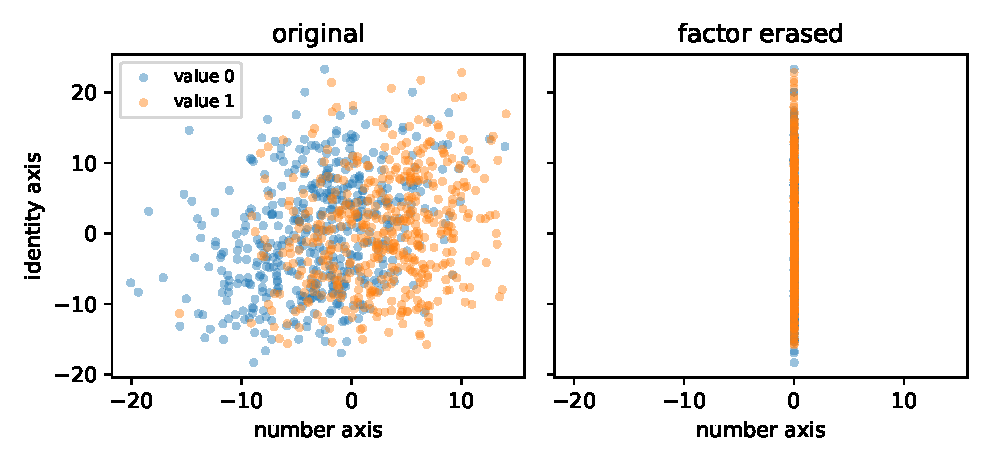
\includegraphics[width=0.92\linewidth]{figures/FD3_erase_canine_number.pdf}
  \caption{Held-out forms before (left) and after (right) linearly erasing the
  number factor, on the factor and identity axes. The factor classes separate
  originally and intermix after erasure; lexical structure is preserved.}
  \label{fig:erase}
\end{figure}

% ===================================================================== %
\section{The Subspace Is Causally Used---and Only When Trained}
\label{sec:causal}

So far the matrix is geometry: it shows the factor is \emph{decodable} and linearly
\emph{removable}. The random-network control warns that decodability alone is weak
evidence about a trained model. The decisive question is therefore behavioural---does
the model \emph{use} the subspace?---and it is the one place the random network should
diverge. We test it with a causal intervention on morphological agreement, the
standard behavioural probe for whether a model represents a feature functionally
\citep{linzen2016assessing,goldberg2019assessing}, made causal by erasing the
candidate subspace and re-measuring the behaviour
\citep{elazar2021amnesic,ravfogel2021counterfactual}.

\paragraph{Set-up.}
We use Hebrew subject--verb and modifier agreement, read off \emph{the model's own
masked-language-model head}---no probe is trained, so there is no classifier to
fish a metric from. Each item is a minimal pair (a correctly- and an
incorrectly-inflected single-token verb form completing a number- or
gender-marked subject context); agreement accuracy is the fraction of items on
which the head assigns higher probability to the grammatical form. We then fit a
LEACE eraser for each feature on subject-context representations and apply it to
the hidden state before the head. We cross two agreement tasks (number, gender) with
four interventions---none, erase-number, erase-gender, and a rank-matched
\emph{random} direction---and run the whole thing on the pretrained model and on a
random-init model of the same architecture.

\paragraph{A double dissociation, only in the trained model.}
Table~\ref{tab:causal} is the result. In the pretrained model, erasing
\emph{number} drives \emph{number} agreement from $0.97$ to exactly chance while
leaving \emph{gender} agreement intact ($0.94\!\to\!0.93$); erasing \emph{gender}
does the mirror image ($0.94\!\to\!0.50$ for gender, $0.97\!\to\!0.96$ for number).
The rank-matched random direction harms neither, so the collapse is the targeted
feature's removal, not generic damage. And the random-init model has no agreement
to break: every cell sits at chance regardless of intervention. The dissociation is
stable across seeds (standard deviations $\le 0.01$).

\begin{table}[t]
  \centering
  \small
  % Generated by disentangle/results.py -- do not edit by hand.
\begin{tabular}{llcccc}
\toprule
& & \multicolumn{4}{c}{Agreement accuracy (chance .5) after erasing} \\
\cmidrule(lr){3-6}
Model & Agreement task & none & $-$number & $-$gender & $-$random \\
\midrule
pretrained AlephBERT & number agr.\ & $0.967\pm0.000$ & $0.500\pm0.000$ & $0.957\pm0.000$ & $0.968\pm0.000$ \\
 & gender agr.\ & $0.940\pm0.000$ & $0.933\pm0.000$ & $0.500\pm0.000$ & $0.939\pm0.001$ \\
\midrule
random-init AlephBERT & number agr.\ & $0.496\pm0.007$ & $0.500\pm0.000$ & $0.498\pm0.005$ & $0.493\pm0.003$ \\
 & gender agr.\ & $0.498\pm0.003$ & $0.496\pm0.005$ & $0.500\pm0.000$ & $0.497\pm0.001$ \\
\bottomrule
\end{tabular}

  \caption{Causal agreement test (mean${}\pm{}$SD over three seeds). Agreement
  accuracy is read from AlephBERT's masked-LM head (no trained probe). In the
  pretrained model each eraser collapses \emph{only} its own agreement task to
  chance while a rank-matched random direction spares both; the random-init model
  has no agreement to begin with. Geometry is necessary for separability, but only
  the trained model \emph{uses} the subspace.}
  \label{tab:causal}
\end{table}

This is the complement to the random-network control. The control showed the
\emph{separability geometry} is largely surface-carried and present without training;
the intervention shows the \emph{function}---using that geometry to drive
agreement---is learned, feature-specific, and absent from the untrained network. The
same subspace the instrument isolates is the one the model causally relies on, and
the random network is a foil that has the shape without the use.

% ===================================================================== %
\section{Cross-Lingual Replication}
\label{sec:crosslang}

To show the instrument is not Syriac-specific, Table~\ref{tab:crosslang} runs the
identical design on Hebrew (AlephBERT) and Arabic (CAMeLBERT) with factors and
minimal pairs drawn from UniMorph. On native Hebrew the matrix is not only clean but
sharper than the Syriac cells: number is decodable at $0.92$ and erases to chance
($0.50$) while identity retrieval survives ($0.64\!\to\!0.73$), and erasing identity
sends retrieval to $0.00$ while number stays at $0.88$; gender behaves identically.
Arabic shows the same clean off-diagonal ($0.88\!\to\!0.55$ for number under
erasure with identity surviving, retrieval $0.37\!\to\!0.00$ under lexeme erasure
with number retained). One practical caveat fixes the surface for Arabic: CAMeLBERT
is trained on undiacritised Classical Arabic and its tokeniser maps every
fully-vocalised UniMorph form to a single \texttt{<unk>}, so we feed it the
undiacritised surface it actually reads---which makes Arabic parallel to unvocalised
Hebrew and leaves the consonantal control vacuous in both. The grids and chance
levels are in Table~\ref{tab:grids}. That the same balanced-grid, cross-erasure
measurement transfers from a zero-resource abjad to two well-resourced relatives,
across byte, subword, and transfer encoders, supports treating templatic morphology
as a general instrument for this question.

\begin{table}[t]
  \centering
  \small
  % Generated by disentangle/results.py -- do not edit by hand.
\begin{tabular}{llcccccc}
\toprule
& & \multicolumn{3}{c}{Factor acc.\ (chance .5)} & \multicolumn{3}{c}{Lexeme \textsc{nn}} \\
\cmidrule(lr){3-5}\cmidrule(lr){6-8}
Language & Factor & orig.\ & $-$factor & $-$lexeme & orig.\ & $-$factor & $-$lexeme \\
\midrule
Hebrew & number & $0.918\pm0.006$ & $0.495\pm0.020$ & $0.876\pm0.019$ & $0.640\pm0.025$ & $0.725\pm0.023$ & $0.002\pm0.001$ \\
Hebrew & gender & $0.899\pm0.006$ & $0.511\pm0.006$ & $0.871\pm0.018$ & $0.633\pm0.023$ & $0.713\pm0.014$ & $0.001\pm0.001$ \\
\bottomrule
\end{tabular}

  \caption{Cross-lingual replication (model-facing surface; mean${}\pm{}$SD over
  five seeds). The same cross-erasure selectivity holds for native Hebrew and
  Arabic; on Hebrew it is sharper than for Syriac.}
  \label{tab:crosslang}
\end{table}

\begin{table}[t]
  \centering
  \small
  % Generated by disentangle/results.py -- do not edit by hand.
\begin{tabular}{llrr}
\toprule
Language & Factor & Lemma pairs & Chance (\textsc{nn}) \\
\midrule
Syriac & number & 1,512 & 0.0022 \\
Syriac & gender & 511 & 0.0065 \\
Syriac & state & 295 & 0.0114 \\
Hebrew & number & 1,174 & 0.0028 \\
Hebrew & gender & 1,176 & 0.0028 \\
\bottomrule
\end{tabular}

  \caption{Balanced grids. Each lexeme contributes one form per factor value;
  chance for lexeme \textsc{nn} retrieval is $1/|\text{test lexemes}|$.}
  \label{tab:grids}
\end{table}

% ===================================================================== %
\section{Discussion}
\label{sec:discussion}

The headline is easy to overstate, and the random-network control is what keeps it
honest. Frozen encoders---byte, subword, transfer, and even untrained---store a
Semitic language's morphosyntactic pattern in a linear subspace separable from
lexical identity, cleanly and symmetrically. But because an untrained network of the
same shape does the same, the right reading is not that pretraining \emph{discovers}
the factorisation; it is that templatic morphology marks its factors in surface
positions that a generic byte feature map already renders linearly separable.
Pretraining and in-language adaptation then act as a refinement: they raise
decodability and move the number signal further into the vowels, where the
orthography actually carries it. For interpretability practice the lesson is the
familiar one of control tasks, made measurable by a clean instrument: a clean
erasure matrix is necessary but not sufficient evidence about a \emph{learned}
representation.

The positive contribution is methodological. Where disentanglement studies usually
rely on synthetic generative factors, a labelled templatic lexicon supplies real,
naturally occurring, independently labelled factors at scale, and the same design
runs across languages and encoders without modification. And the pairing of a
random-network control with a causal agreement intervention is what lets the
instrument separate the two questions it is easy to conflate: whether a feature is
\emph{linearly present} (it is, largely from the surface) and whether the model
\emph{uses} it (it does, and only after training). The geometry it exposes is also
linguistically legible: the consonantal control recovers, from the model's internal
arrangement, the same division of labour between vowels and consonants that a grammar
of the script would state.

% ===================================================================== %
\section{Limitations}
\label{sec:limitations}

The selectivity matrix is observational geometry: on its own it shows that factor
and identity occupy separable linear subspaces, not that a computation uses them.
The agreement intervention (\S\ref{sec:causal}) supplies the causal step for two
features in one language; we have not shown the same for every factor or language,
and the behavioural test relies on single-token agreement forms, which filters the
item set. Effect sizes for the geometry are modest---the Hebrew-transfer number
probe is only $\sim$$0.62$, and identity retrieval is well below ceiling---so the
matrix supports qualitative separability claims rather than precise capacity
estimates. We test binary contrasts on three factors, so ``word $=$ root $\times$
pattern'' as a full algebra remains aspirational. The Syriac labels are the
New-Testament-scoped SEDRA lexicon; the UniMorph grids inherit that resource's
coverage and its mix of inflectional types. The identity-erasure direction is
transductive (fit on the test lexemes whose retrieval it measures), appropriate for
a per-form quantity but weaker than the inductive factor-erasure direction. Finally,
the random-network control shows the surface baseline is high; we therefore report
what adaptation adds as a
small, directional effect rather than a large one.

% ===================================================================== %
\section{Conclusion}
\label{sec:conclusion}

Templatic morphology, with a morphological lexicon, is a clean and reusable
instrument for the disentanglement question: it yields balanced, decorrelated factor
labels and a symmetric cross-erasure matrix that needs no model training. With it we
find that frozen encoders linearly separate morphosyntactic pattern from lexical
identity across three Semitic languages---but that a random-initialised network of
the same architecture does too, so the separability is largely surface-carried, with
pretraining and adaptation adding a measurable sharpening and a relocation of number
into the vocalic channel. A causal agreement intervention then shows that, despite
the shared geometry, only the trained model \emph{uses} the subspace: erasing a
feature collapses exactly its own agreement and nothing else, while the random
network has no agreement to lose. Pairing a random-network control with a behavioural
intervention is, we argue, the point---the instrument measures both whether a feature
is present and whether it is used.

% ===================================================================== %
\section*{Reproducibility}
The probes, erasers (INLP and a \textsc{NumPy} LEACE), the balanced-grid
construction, the cross-language UniMorph loader, the agreement intervention on the
masked-LM head, and the table/figure generators are released. The Syriac labels are
regenerated locally from a user-provided SEDRA
source and the UniMorph data is downloaded on demand; neither is redistributed.
Every number traces to a single regenerable manifest.

\bibliographystyle{plainnat}
\bibliography{references}

\end{document}
